\chapter{Reproduction asexuée et clonage chez les plantes}\label{ch:b2:asexual-reproduction}

Dans une vallée de l'Utah se dresse une forêt de quarante-sept mille
troncs de trembles qui ne forme qu'une seule plante~: chaque tronc est
issu du même système racinaire, chaque cellule porte le même génome, et
l'individu, âgé de quelque quatorze mille ans, pèse six mille tonnes.
Toutes les fraises d'une barquette d'une même variété sont des morceaux
d'une seule plante multipliée par stolons~; toutes les bananes Cavendish
de la planète sont des boutures de boutures d'une seule plante. Les
plantes, contrairement à la plupart des animaux, peuvent produire de
nouveaux individus sans sexualité --- à partir d'une tige, d'une racine,
d'une feuille, d'une seule cellule dans un flacon. Ce chapitre examine
comment elles y parviennent, comment les producteurs en tirent parti, et
ce qu'il en coûte à une lignée de renoncer à la \omterm{def:b2:meiosis-heredity:meiosis}{méiose} et à la
fécondation~: la question de savoir pourquoi la sexualité existe.

\section{La multiplication végétative}

\begin{definition}[Clone, génet, ramet]\label{def:b2:asexual-reproduction:clone}
\index{clone}\index{genet@génet}\index{ramet}\index{multiplication vegetative@multiplication végétative}
La \emph{reproduction asexuée} produit de nouveaux individus à partir
d'un seul parent, par mitoses uniquement, sans \omterm{def:b2:meiosis-heredity:meiosis}{méiose} ni fécondation~:
les descendants forment un \emph{clone}, génétiquement identique au
parent et identiques entre eux, aux \omterm{def:b2:genome-diversification:mutation}{mutations} somatiques accumulées
près. Chez les plantes, la forme habituelle en est la
\emph{multiplication végétative}, dans laquelle une partie du corps ---
tige, racine, feuille --- s'enracine et devient une plante séparée. Un
\emph{génet} est l'individu génétique, tout ce qui est issu d'un même
zygote~; un \emph{ramet} en est une unité physiologiquement séparée. Une
planche de fraisiers peut contenir un millier de ramets d'un même
génet~; la forêt de trembles est un seul génet. La multiplication
végétative est possible parce que les cellules végétales conservent la
capacité de se diviser et de former n'importe quel organe --- elles
sont \emph{totipotentes} --- et parce que les plantes croissent à partir
de méristèmes qui peuvent être réveillés presque partout.
\end{definition}

\begin{proposition}[Les organes de la multiplication végétative]\label{prop:b2:asexual-reproduction:organs}
\index{stolon}\index{rhizome}\index{tubercule}\index{bulbe}
Les plantes ont inventé la même astuce à partir de chaque organe. À
partir des tiges~: les \emph{coulants} ou \emph{stolons}, tiges
horizontales rampant sur le sol qui s'enracinent à leurs nœuds
(fraisier, renoncule rampante)~; les \emph{rhizomes}, tiges souterraines
horizontales qui se ramifient et se fragmentent (chiendent, iris,
gingembre, \omterm{def:b2:plant-life-cycles:fern}{fougère} aigle)~; les \emph{tubercules}, extrémités renflées de
tiges souterraines qui stockent de l'amidon et portent des bourgeons,
les «~yeux~» (pomme de terre)~; les \emph{bulbes solides}, bases de tiges
verticales renflées (crocus)~; les \emph{bulbilles}, petits bulbes
formés à l'aisselle des feuilles ou dans l'inflorescence (ail, certains
oignons). À partir des feuilles~: les \emph{bulbes}, bourgeons enveloppés
de feuilles charnues de réserve qui se divisent en bulbes fils (oignon,
tulipe)~; des plantules formées le long du bord des feuilles, pourvues
de racines, qui s'en détachent (\emph{Kalanchoe}). À partir des
racines~: les \emph{drageons}, pousses qui s'élèvent de racines
horizontales (tremble, prunellier, framboisier). Par
\emph{fragmentation}~: un morceau de branche de saule emporté par l'eau
qui s'enracine, une fronde de lentille d'eau qui se divise. Dans tous
les cas, un organe de réserve ou un méristème est transporté à courte
distance, et la plante fille commence sa vie avec une provision de
nourriture qu'aucune \omterm{def:b2:angiosperm-reproduction:seed}{graine} ne peut égaler.
\end{proposition}

\begin{omfigure}
\begin{tikzpicture}[every node/.style={font=\scriptsize}]
  % runner
  \begin{scope}
    \draw[thick] (0,0) -- (3.6,0);
    \foreach \x in {0,1.8} { \draw[thick, omExo!70!black, fill=omExo!30] (\x,0) .. controls (\x-0.3,0.6) and (\x+0.3,0.6) .. (\x,0); \foreach \a in {60,90,120} \draw[thick, omExo!70!black] (\x,0) -- ++(\a:0.7); \draw[gray] (\x,0) -- ++(-100:0.4) (\x,0) -- ++(-70:0.4); }
    \draw[thick, omThm] (0.2,0.15) .. controls (0.9,0.55) and (1.2,0.55) .. (1.8,0.1);
    \draw[thick, omThm] (2.0,0.15) .. controls (2.7,0.55) and (3.0,0.55) .. (3.5,0.1);
    \draw[thick, omExo!70!black] (3.5,0.1) -- ++(80:0.4); \draw[gray] (3.5,0.1) -- ++(-80:0.3);
    \node[below, align=center] at (1.8,-0.55) {stolon (fraisier)~:\\une tige horizontale s'enracine à ses nœuds};
  \end{scope}
  % rhizome and tuber
  \begin{scope}[xshift=5.2cm]
    \draw[gray, dashed] (-0.2,0) -- (3.8,0);
    \draw[very thick, omProp!80!black] (0,-0.5) -- (3.4,-0.5);
    \foreach \x in {0.6,2.0} \draw[thick, omExo!70!black] (\x,-0.5) -- (\x,0.7) (\x,0.3) -- ++(40:0.4) (\x,0.3) -- ++(140:0.4);
    \draw[thick, omProp!80!black, fill=omProp!40] (3.4,-0.5) ellipse (0.45 and 0.3);
    \foreach \p in {(3.2,-0.3),(3.6,-0.35),(3.7,-0.6)} \fill[omThm] \p circle (0.04);
    \foreach \x in {0.3,1.3,2.5} \draw[gray] (\x,-0.5) -- (\x,-0.9);
    \node[below, align=center] at (1.8,-1.05) {rhizome et tubercule (pomme de terre)~:\\tiges souterraines,\\bourgeons (yeux) sur le tubercule};
  \end{scope}
  % bulb
  \begin{scope}[xshift=12.2cm]
    \draw[thick, fill=omExo!15] (0,-0.9) .. controls (-0.9,-0.6) and (-0.9,0.9) .. (0,1.0) .. controls (0.9,0.9) and (0.9,-0.6) .. (0,-0.9);
    \foreach \r in {0.55,0.35} \draw[thick] (0,-0.75) .. controls (-\r,-0.5) and (-\r,0.6) .. (0,0.8) .. controls (\r,0.6) and (\r,-0.5) .. (0,-0.75);
    \fill[omExo!60!black] (-0.1,-0.75) rectangle (0.1,0.3);
    \draw[thick, omThm, fill=omThm!30] (0.35,-0.5) ellipse (0.15 and 0.3);
    \foreach \x in {-0.3,0,0.3} \draw[gray] (\x,-0.9) -- (\x,-1.25);
    \node[below, align=center] at (0,-1.3) {bulbe (oignon)~:\\feuilles charnues,\\un bulbe fils (en rouge)};
  \end{scope}
\end{tikzpicture}

{\small Trois organes de \omterm{def:b2:asexual-reproduction:clone}{multiplication végétative}~: des stolons qui
s'enracinent à leurs nœuds, une tige souterraine qui se renfle en
tubercule, et un bulbe qui bourgeonne un bulbe fils. Dans chaque cas, un
bourgeon voyage avec sa nourriture.}
\end{omfigure}

\begin{omfigure}
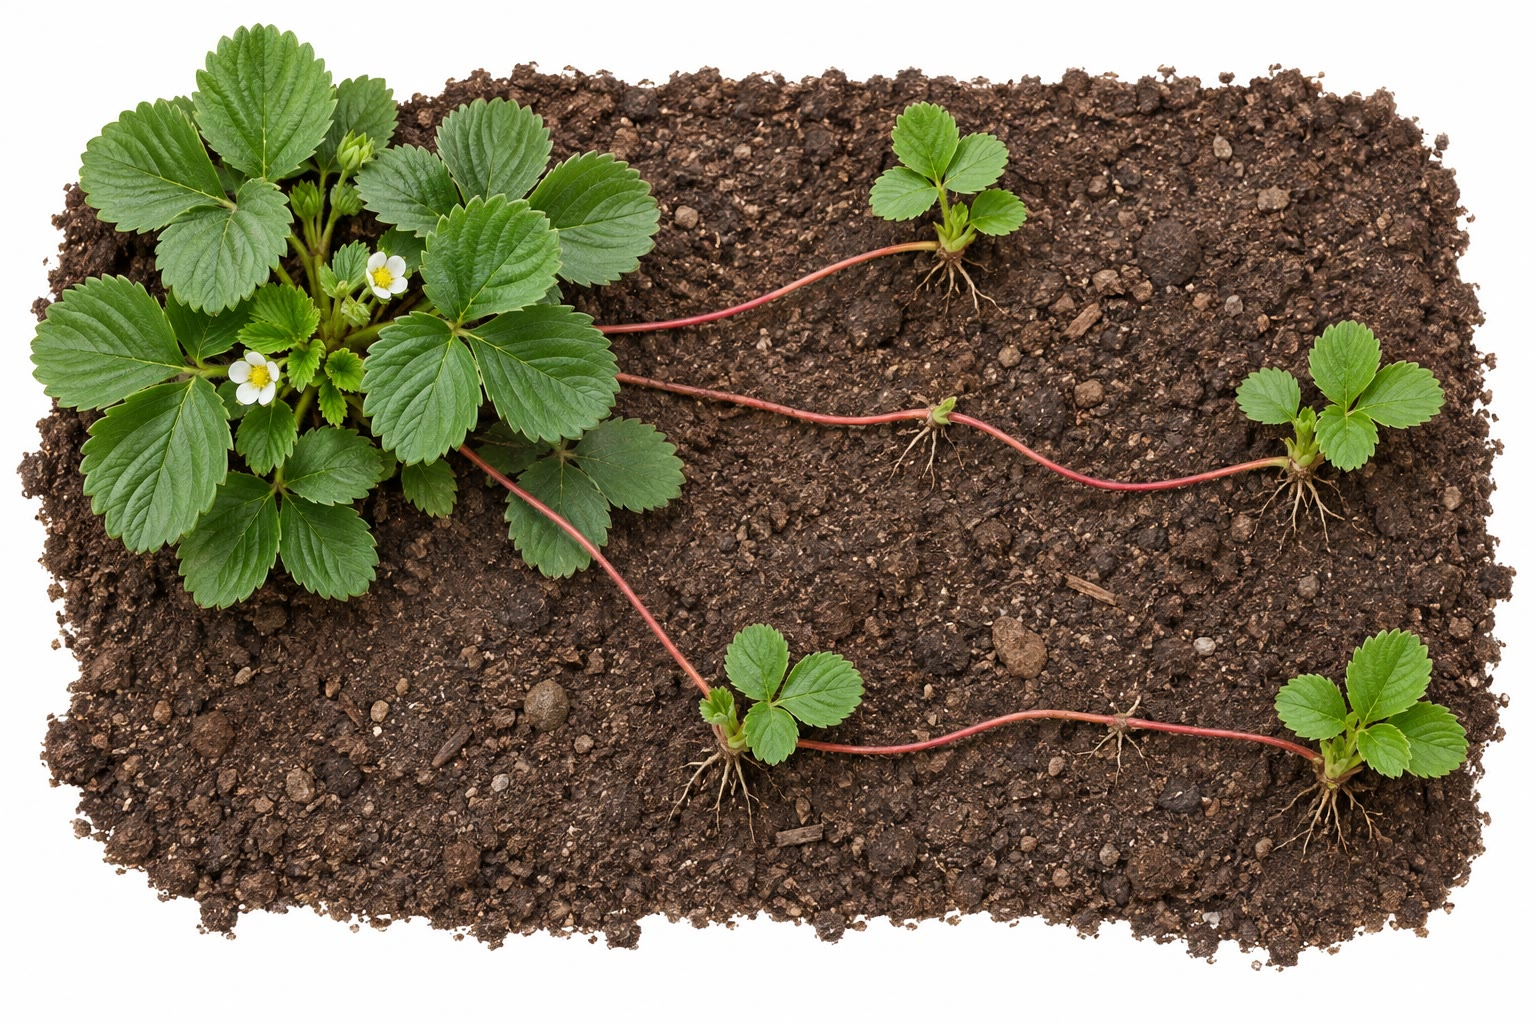
\includegraphics[width=0.46\linewidth]{images/book4/ai/b4-07-strawberry-runners.jpg}\hspace{0.03\linewidth}
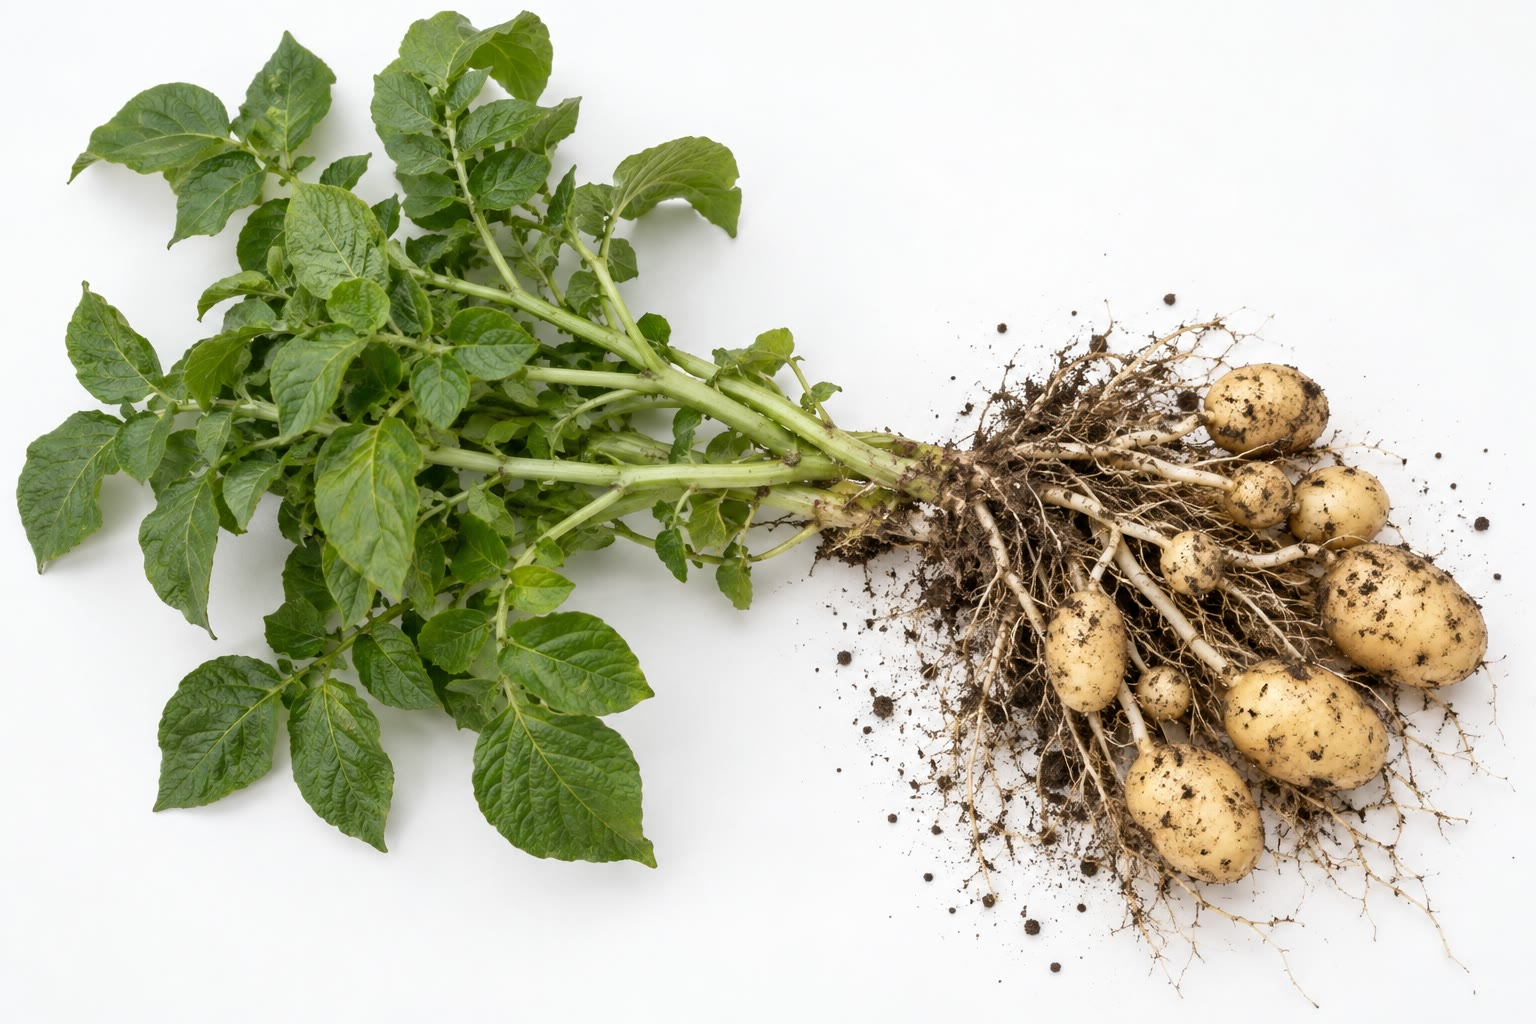
\includegraphics[width=0.46\linewidth]{images/book4/ai/b4-07-potato-tubers.jpg}

{\small À gauche~: un fraisier et les plantes filles qui s'enracinent le
long de ses stolons. À droite~: un plant de pomme de terre sorti de
terre, ses tubercules suspendus à des stolons --- chaque tubercule est un
morceau de tige qui donnera une plante génétiquement identique à
celle-ci.}
\end{omfigure}

\begin{theorem}[La géométrie d'un clone qui s'étend]\label{thm:b2:asexual-reproduction:spread}
\index{croissance clonale}
Un \omterm{def:b2:asexual-reproduction:clone}{génet} dont chaque \omterm{def:b2:asexual-reproduction:clone}{ramet} produit chaque année $m$ filles enracinées,
toutes survivantes, croît en nombre selon $N(t) = N_0 (1 + m)^t$ ---
une croissance exponentielle sans aucune sexualité --- jusqu'à ce que
les \omterm{def:b2:asexual-reproduction:clone}{ramets} remplissent l'espace à leur densité maximale $d$ (\omterm{def:b2:asexual-reproduction:clone}{ramets} par
unité de surface), après quoi le \omterm{def:b2:asexual-reproduction:clone}{clone} progresse comme un front. Un
\omterm{def:b2:asexual-reproduction:clone}{clone} qui étend ses stolons en ligne droite à la vitesse $v$ a, au bout
de $t$ années, un rayon $vt$, et le nombre de \omterm{def:b2:asexual-reproduction:clone}{ramets} croît comme
$\pi d (vt)^2$~: de façon quadratique, et non exponentielle. Un fraisier
qui émet des stolons de \qty{0.5}{m} par an a un rayon de \qty{5}{m} au
bout de dix ans~; le \omterm{def:b2:asexual-reproduction:clone}{clone} de trembles du début du chapitre,
\qty{43}{ha}, a un rayon de quelque \qty{370}{m} et, pour une
progression nette de quelques centimètres par an, un âge de l'ordre de
$10^{4}$ ans --- ce qui concorde avec l'âge estimé d'après le recul des
glaciers.
\end{theorem}
\begin{proof}
Chaque année, chaque \omterm{def:b2:asexual-reproduction:clone}{ramet} est remplacé par lui-même et $m$ filles, soit
un facteur $1 + m$~; $t$ années donnent $(1 + m)^t$. Une fois l'intérieur
rempli, seuls les \omterm{def:b2:asexual-reproduction:clone}{ramets} situés en bordure trouvent de la place, et la
bordure progresse à la vitesse des stolons $v$~; la surface vaut
$\pi(vt)^2$ et le nombre de \omterm{def:b2:asexual-reproduction:clone}{ramets} est la surface multipliée par la
densité.
\end{proof}

\begin{example}[Les organismes les plus âgés]\label{ex:b2:asexual-reproduction:oldest}
Le \omterm{def:b2:asexual-reproduction:clone}{clone} de trembles Pando (Utah) couvre \qty{43}{ha} avec environ
\num{47000} troncs, qui vivent chacun un siècle environ et sont remplacés
par des drageons issus des mêmes racines~; le \omterm{def:b2:asexual-reproduction:clone}{génet} pourrait avoir plus
de dix mille ans. Un \omterm{def:b2:asexual-reproduction:clone}{clone} de la posidonie (\emph{Posidonia}) en
Méditerranée s'étend sur \qty{15}{km} et pourrait avoir cent mille ans~;
un anneau de créosotier du désert de Mojave a été daté de \num{11700}
ans, les tiges centrales mourant à mesure que l'anneau s'étend. Dans
tous les cas, ce qui est ancien, c'est le \omterm{def:b2:asexual-reproduction:clone}{génet}~; aucune cellule n'y a
plus de quelques décennies, et le génome a été copié des milliers de
fois.
\end{example}

\section{Des graines sans sexualité, et des animaux sans père}

\begin{definition}[Apomixie]\label{def:b2:asexual-reproduction:apomixis}
\index{apomixie}\index{parthenogenese@parthénogenèse}
L'\emph{apomixie} est la production de \omterm{def:b2:angiosperm-reproduction:seed}{graines} sans fécondation~: un
embryon se développe à partir d'une oosphère non réduite (la cellule
mère des \omterm{def:b2:plant-life-cycles:heterospory}{macrospores} saute la \omterm{def:b2:meiosis-heredity:meiosis}{méiose}) ou directement à partir d'une
cellule du nucelle, et la \omterm{def:b2:angiosperm-reproduction:seed}{graine} porte le \omterm{def:b2:meiosis-heredity:vocabulary}{génotype} de la mère. Le
pissenlit, les épervières, la ronce, le pâturin des prés et de nombreux
agrumes procèdent ainsi~; la \omterm{def:b2:angiosperm-reproduction:seed}{graine} d'agrume contient souvent plusieurs
embryons, l'un sexué et les autres copies nucellaires de la mère.
L'apomixie conserve la \omterm{def:b2:angiosperm-reproduction:seed}{graine} --- sa dispersion, sa \omterm{def:b2:angiosperm-reproduction:seed}{dormance} et son
tégument --- et supprime la \omterm{def:b2:meiosis-heredity:meiosis}{méiose}, si bien qu'un \omterm{def:b2:meiosis-heredity:vocabulary}{génotype} bien adapté
est diffusé sans changement~; la plupart des apomictiques sont des
\omterm{def:b2:genome-diversification:polyploidy}{polyploïdes} d'origine hybride dont la \omterm{def:b2:meiosis-heredity:meiosis}{méiose} échouerait de toute façon.
Son équivalent animal est la \emph{parthénogenèse}, le développement à
partir d'un ovocyte non fécondé~: obligatoire chez certains lézards et
chez les rotifères bdelloïdes, qui n'ont plus de mâles depuis des
dizaines de millions d'années~; cyclique chez les pucerons et les
daphnies, qui se multiplient par parthénogenèse tout l'été, une femelle
donnant naissance à des filles vivantes qui portent déjà leurs propres
embryons, et passent à l'automne à une génération sexuée qui pond des
œufs d'hiver.
\end{definition}

\begin{omfigure}
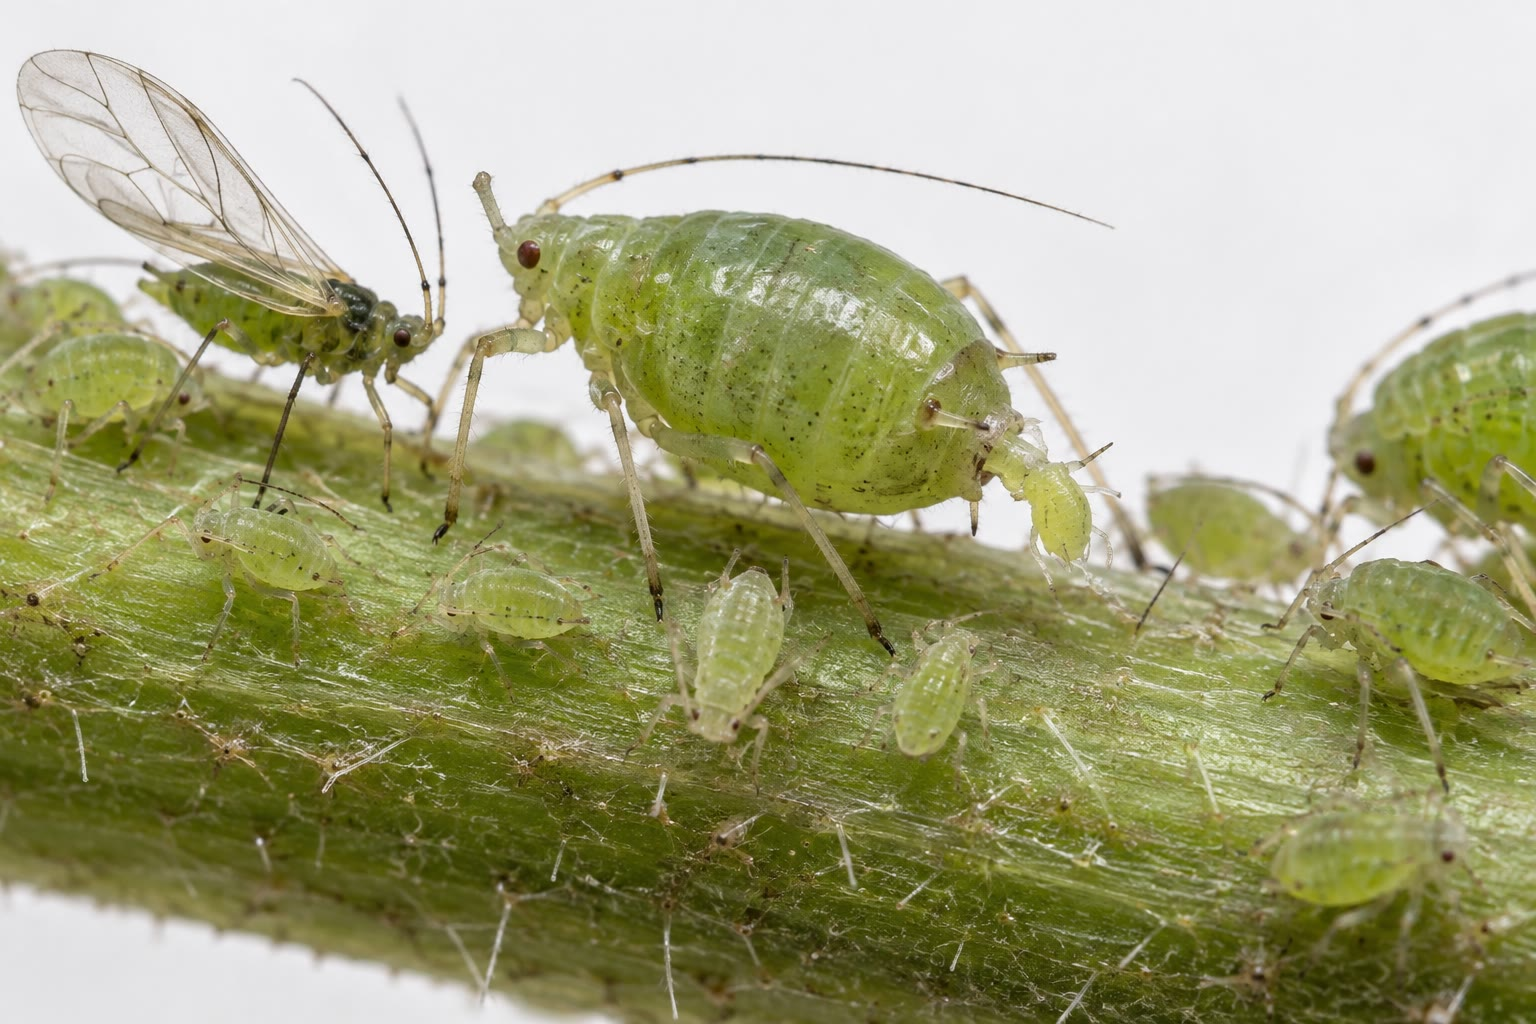
\includegraphics[width=0.55\linewidth]{images/book4/ai/b4-07-aphids.jpg}

{\small Des pucerons sur une tige~: une femelle parthénogénétique aptère
donnant naissance à une fille vivante, des larves de plusieurs âges et
un migrant ailé --- la croissance exponentielle d'un été sans un seul
mâle.}
\end{omfigure}

\begin{example}[Un été de pucerons]\label{ex:b2:asexual-reproduction:aphids}
Un puceron parthénogénétique atteint la maturité en huit jours environ
et produit quelque cinq filles par jour pendant deux semaines~; les
filles naissent déjà gestantes (les embryons commencent à se développer
à l'intérieur des embryons de la mère). Avec un \omterm{def:b2:unicellular-diversity:division}{temps de génération}
voisin de dix jours et un taux net d'accroissement d'environ \num{50}
par génération, une seule fondatrice en avril pourrait, sans frein,
laisser $50^{12} \approx 2\times 10^{20}$ descendants en octobre ---
une masse supérieure à celle de la Terre. Coccinelles, chrysopes, guêpes
parasitoïdes, champignons et pluie maintiennent leur nombre à quelques
milliers par plante, et la génération sexuée d'automne réinitialise le
\omterm{def:b2:asexual-reproduction:clone}{clone} en œufs recombinés avant l'hiver.
\end{example}

\section{Le clonage par le producteur}

\begin{proposition}[Bouturage, marcottage, greffage]\label{prop:b2:asexual-reproduction:horticulture}
\index{bouture}\index{greffe}\index{porte-greffe}
Une \emph{bouture} est un fragment de tige, de racine ou de feuille que
l'on amène à s'enraciner~: l'extrémité coupée forme un cal de cellules en
division d'où naissent des méristèmes racinaires, avec l'aide de l'auxine
(l'hormone de bouturage) et de l'humidité. Le \emph{marcottage} fait
s'enraciner une branche encore attachée et ne la sépare qu'ensuite. La
\emph{greffe} unit une pousse d'une plante (le \emph{greffon}) à la tige
enracinée d'une autre (le \emph{porte-greffe})~: les deux cambiums sont
pressés l'un contre l'autre, un cal comble la plaie, et de nouveaux
xylème et phloème se raccordent en quelques semaines. La greffe est une
chimère --- les racines gardent le génome du porte-greffe, la pousse
fructifère celui du greffon --- et elle ne réussit qu'entre plantes
apparentées (espèces d'un même genre, parfois d'une même famille), car
les tissus doivent se reconnaître mutuellement. Toutes les variétés de
pommier, de poirier, de cerisier, d'agrumes et de vigne sont multipliées
par greffe~: une variété nommée est un seul \omterm{def:b2:asexual-reproduction:clone}{génet}, maintenu en vie
pendant des siècles par des greffons (les reinettes remontent au
\textsc{xvi}\textsuperscript{e} siècle), et le porte-greffe est choisi
pour le sol, la résistance aux maladies et la taille d'arbre voulue ---
les porte-greffes nanisants donnent les petits arbres des vergers
modernes.
\end{proposition}

\begin{proposition}[Micropropagation et totipotence]\label{prop:b2:asexual-reproduction:tissueculture}
\index{micropropagation}\index{totipotence}\index{cal}
Toute cellule végétale vivante pourvue d'un noyau peut, en principe,
régénérer une plante entière. En \emph{culture de tissus}, un fragment
de tissu stérilisé (un \emph{explant}~: un apex de tige, un disque de
feuille, une anthère) est placé sur un milieu gélosé contenant du sucre,
des minéraux, des vitamines et des hormones. Avec de l'auxine et de la
cytokinine en proportions équilibrées, les cellules se dédifférencient
en un \emph{cal}, une masse de cellules non spécialisées en division~;
avec plus de cytokinine que d'auxine, le cal forme des tiges, avec plus
d'auxine que de cytokinine, il forme des racines, et chez certaines
espèces il forme des \emph{embryons somatiques} --- des embryons
complets sans oosphère. Les tiges sont coupées et repiquées toutes les
quelques semaines, en se multipliant chaque fois par un facteur de trois
à dix, si bien qu'un méristème donne un million de plantules en un an.
Comme les virus sont en retard sur l'apex en croissance, un méristème
de tige de moins d'un millimètre est en général indemne de virus, même
chez une plante infectée~: la \emph{culture de méristèmes} permet
d'assainir les stocks de pomme de terre, de fraisier, de bananier et
d'orchidées. La méthode est la preuve pratique de la totipotence, et la
raison pour laquelle une variété végétale peut être vendue par millions
dans les quelques années qui suivent sa création.
\end{proposition}
\begin{proof}[Faits expérimentaux]
Skoog et Miller (1957) cultivèrent du cal de moelle de tabac sur des
milieux présentant différents rapports entre l'auxine et la cytokinine,
récemment découverte~: beaucoup d'auxine donnait des racines, beaucoup de
cytokinine des tiges, un équilibre seulement du cal --- la formation des
organes était réglée par le rapport de deux hormones, et non par une
substance organogène spécifique. Steward (1958) mit en suspension des
cellules isolées et de petits amas issus d'une racine de carotte dans un
flacon rotatif de lait de coco~: certains amas formèrent des structures
semblables à des embryons qui se développèrent en carottes complètes et
fleuries, montrant qu'une cellule différenciée d'un organe mature
conserve, et peut utiliser, tout le programme du développement.
\end{proof}

\begin{omfigure}
\begin{tikzpicture}[every node/.style={font=\scriptsize}, >=stealth]
  \node[draw, rounded corners, fill=omDef!12, align=center] (ex) at (0,0) {explant\\(apex, disque de feuille)};
  \node[draw, rounded corners, fill=omExo!30, align=center] (cal) at (4.6,0) {cal\\auxine $\approx$ cytokinine};
  \node[draw, rounded corners, fill=omExo!30, align=center] (sh) at (8.4,1.2) {tiges\\cytokinine $>$ auxine};
  \node[draw, rounded corners, fill=omExo!30, align=center] (rt) at (8.4,-1.2) {racines\\auxine $>$ cytokinine};
  \node[draw, rounded corners, fill=omDef!12, align=center] (pl) at (12.2,0) {plantules\\acclimatées en terre};
  \draw[->, thick] (ex) -- (cal) node[midway, below, align=center] {milieu\\stérile};
  \draw[->, thick] (cal) -- (sh); \draw[->, thick] (cal) -- (rt);
  \draw[->, thick] (sh) -- (pl); \draw[->, thick] (rt) -- (pl);
  \draw[->, thick, omThm] (sh) .. controls (8.4,2.6) and (5.8,2.6) .. (5.2,0.6);
  \node[omThm, anchor=south] at (6.9,2.3) {repiquage toutes les 4 semaines, $\times 5$};
\end{tikzpicture}

{\small La micropropagation~: un explant est dédifférencié en cal,
orienté vers la formation de tiges ou de racines par le rapport
auxine/cytokinine, et multiplié par des repiquages successifs avant que
les plantules ne soient sevrées en terre.}
\end{omfigure}

\begin{omfigure}
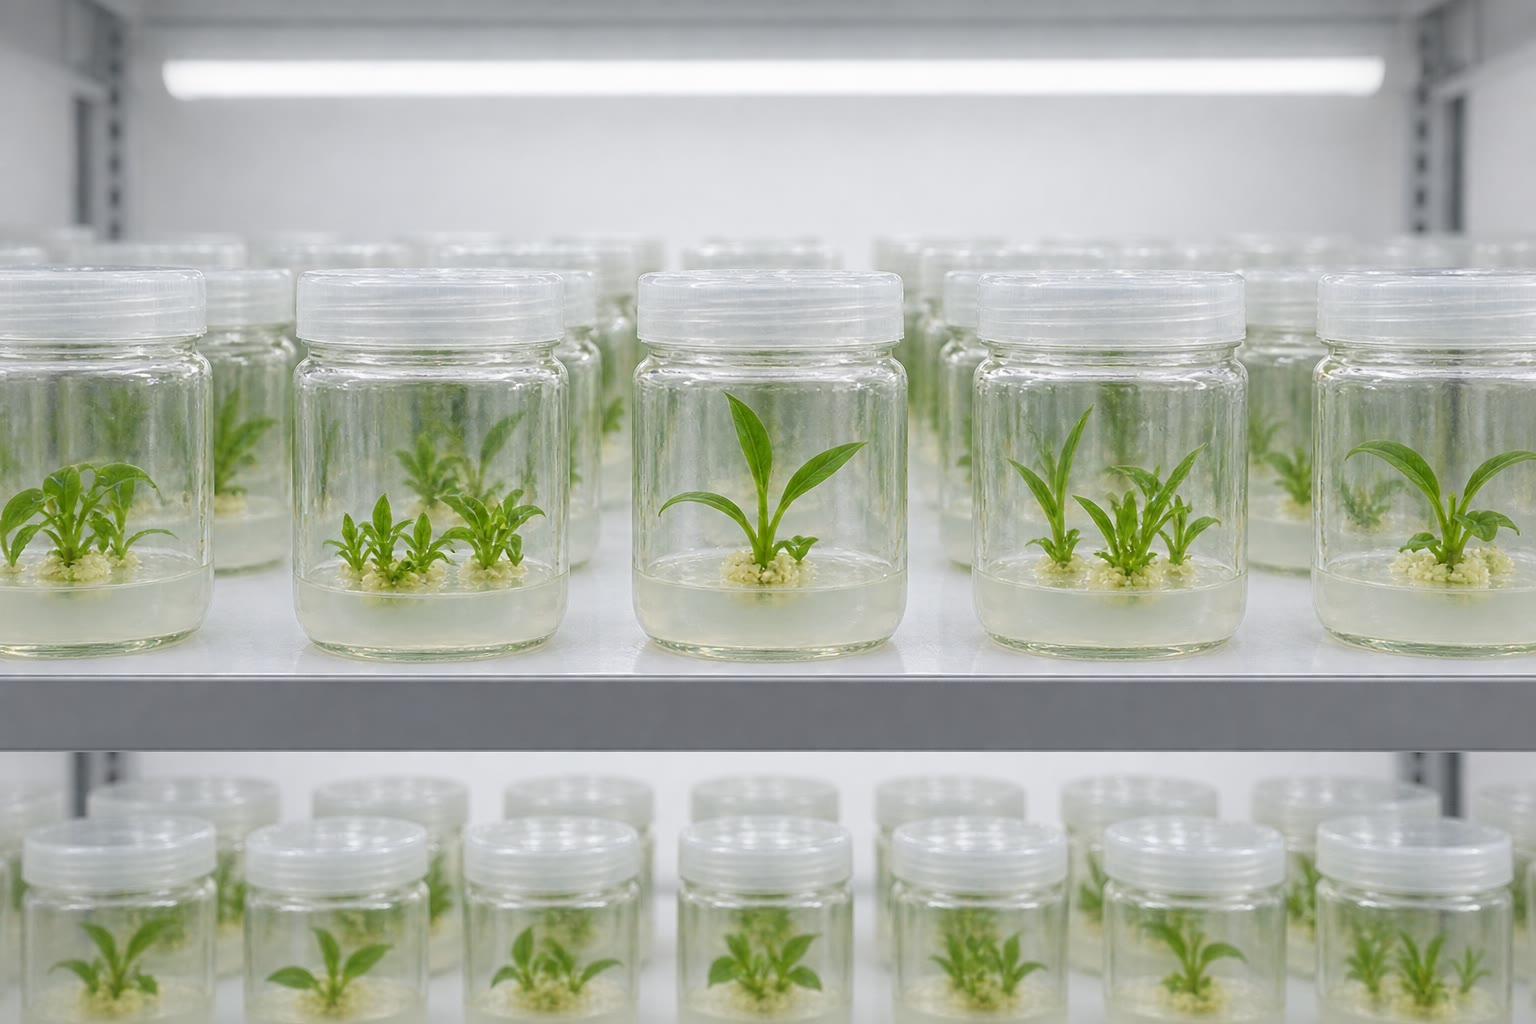
\includegraphics[width=0.6\linewidth]{images/book4/ai/b4-07-tissue-culture.jpg}

{\small Des plantules sur gélose dans une chambre de culture~: chaque
bocal contient un \omterm{def:b2:asexual-reproduction:clone}{clone} de la même variété, multiplié à partir d'un seul
méristème.}
\end{omfigure}

\section{Le coût de la sexualité et le coût de s'en passer}

\begin{theorem}[Le double coût de la sexualité]\label{thm:b2:asexual-reproduction:twofold}
\index{double cout de la sexualite@double coût de la sexualité}
Dans une population où les femelles produisent chacune $F$ descendants,
dont la moitié sont des fils, une femelle mutante asexuée qui produit
$F$ filles, toutes copies d'elle-même, double sa part des femelles de la
génération suivante. Si la lignée asexuée a la fréquence $p$ parmi les
femelles, alors, à la génération suivante,
\[
p' = \frac{2p}{1 + p}, \qquad p_t = \frac{2^t p_0}{1 + (2^t - 1)p_0},
\]
de sorte que, partant d'une sur mille, elle atteint la moitié de la
population en dix générations et la totalité peu après. Toutes choses
égales par ailleurs, la sexualité divise par deux la vitesse à laquelle
une lignée se multiplie --- c'est le prix de la production des mâles.
Puisque la sexualité est pourtant presque universelle, toutes choses ne
sont pas égales~: les lignées sexuées doivent, en moyenne, gagner au
moins un facteur deux grâce à la recombinaison.
\end{theorem}
\begin{proof}
Les femelles asexuées sont au nombre de $pN$ et laissent $FpN$ filles~;
les femelles sexuées sont au nombre de $(1 - p)N$ et laissent
$F(1 - p)N/2$ filles (l'autre moitié sont des fils, qui ne produisent
pas d'ovocytes). La part asexuée des filles vaut
$Fp/(Fp + F(1 - p)/2) = 2p/(1 + p)$. En posant $q = p/(1 -
p)$, la récurrence devient $q' = 2q$, donc $q_t = 2^t q_0$~; en revenant
aux fréquences, on obtient $p_t$. Poser $p_t = \tfrac12$ donne $2^t q_0 = 1$,
c'est-à-dire
$t = \log_2(1/q_0) \approx 10$ pour $p_0 = 10^{-3}$.
\end{proof}

\begin{omfigure}
\begin{tikzpicture}
\begin{axis}[
  width=0.76\linewidth, height=5.6cm,
  axis x line=bottom, axis y line=left,
  xmin=0, xmax=20, ymin=0, ymax=1.05,
  xlabel={générations}, ylabel={fréquence de la lignée asexuée},
  xlabel style={font=\small, at={(axis description cs:0.5,-0.13)}, anchor=north},
  ylabel style={font=\small},
  tick label style={font=\small}, xtick={0,5,10,15,20}, ytick={0,0.5,1},
  legend style={font=\scriptsize, at={(0.5,-0.3)}, anchor=north, draw=none},
  clip=false,
]
\addplot[very thick, omThm, domain=0:20, samples=80] {2^x*0.001/(1+(2^x-1)*0.001)};
\addlegendentry{aucune autre différence~: envahit en 12 générations}
\addplot[very thick, omDef, domain=0:20, samples=80] {0.001*(1.3)^x/(1+(1.3^x-1)*0.001)};
\addlegendentry{les asexués perdent \qty{35}{\%} de valeur sélective (parasites)~: plus lent}
\addplot[very thick, omProp, domain=0:20, samples=80] {0.001*(0.9)^x/(1+(0.9^x-1)*0.001)};
\addlegendentry{les asexués perdent \qty{55}{\%}~: ils ne se répandent jamais}
\end{axis}
\end{tikzpicture}

{\small Le double avantage à l'œuvre. Partant d'une sur mille, une
lignée asexuée sans autre désavantage envahit la population en une
douzaine de générations~; seule une pénalité de valeur sélective d'au
moins la moitié --- due aux parasites, aux \omterm{def:b2:genome-diversification:mutation}{mutations} accumulées ou à une
adaptation plus lente --- la retient.}
\end{omfigure}

\begin{proposition}[À quoi sert la sexualité]\label{prop:b2:asexual-reproduction:whysex}
\index{cliquet de Muller}\index{hypothese de la Reine rouge@hypothèse de la Reine rouge}
Trois bénéfices sont assez grands pour compter. Le \emph{\omterm{prop:b2:asexual-reproduction:whysex}{cliquet de
Muller}}~: dans un \omterm{def:b2:asexual-reproduction:clone}{clone}, toute \omterm{def:b2:genome-diversification:mutation}{mutation} nuisible est héritée par tous
les descendants, et un génome sans \omterm{def:b2:genome-diversification:mutation}{mutation}, une fois perdu par hasard
dans une population finie, ne peut jamais être reconstitué~; le fardeau
monte cran par cran, et les petites populations asexuées dépérissent.
La recombinaison reconstruit des génomes intacts à partir de deux
génomes endommagés. L'\emph{adaptation}~: deux \omterm{def:b2:genome-diversification:mutation}{mutations} utiles
apparues chez des individus différents d'un \omterm{def:b2:asexual-reproduction:clone}{clone} entrent en compétition
et l'une est perdue~; dans une population sexuée, elles se combinent
(Fisher et Muller, années 1930), si bien que les populations sexuées
s'adaptent plus vite lorsque de nombreux gènes doivent changer. La
\emph{Reine rouge}~: les parasites s'adaptent au \omterm{def:b2:meiosis-heredity:vocabulary}{génotype} hôte le plus
commun, et un \omterm{def:b2:asexual-reproduction:clone}{clone}, qui est un seul \omterm{def:b2:meiosis-heredity:vocabulary}{génotype}, est le plus commun de
tous~; des parents sexués font de chaque descendant une serrure
nouvelle. Des escargots, des poissons et des plantes qui possèdent à la
fois des populations sexuées et clonales montrent que les populations
sexuées l'emportent là où les parasites abondent. Les lignées asexuées
qui prospèrent --- pissenlits, rotifères bdelloïdes, la plupart des
\omterm{def:b2:asexual-reproduction:clone}{clones} cultivés --- sont soit jeunes, soit des hybrides \omterm{def:b2:genome-diversification:polyploidy}{polyploïdes} qui
portent leur propre variation, soit maintenues par un producteur qui tue
leurs parasites à leur place.
\end{proposition}

\begin{example}[Des monocultures d'un clone]\label{ex:b2:asexual-reproduction:monoculture}
Dans les années 1840, la plus grande partie de la récolte de pommes de
terre de l'Irlande était une seule variété clonale, la Lumper~; l'oomycète
\emph{Phytophthora infestans}, arrivé en 1845, rencontra un pays de
plantes génétiquement identiques et uniformément sensibles, et détruisit
la récolte trois années de suite. La banane d'exportation mondiale
jusqu'aux années 1950 était un seul \omterm{def:b2:asexual-reproduction:clone}{clone}, la Gros Michel, éliminée des
plantations d'Amérique centrale par un champignon du sol~; sa
remplaçante, la Cavendish, est elle aussi un seul \omterm{def:b2:asexual-reproduction:clone}{clone} et disparaît
aujourd'hui, plantation après plantation, sous l'effet d'une nouvelle
souche du même champignon, contre laquelle elle n'a aucune variation à
opposer. Un \omterm{def:b2:asexual-reproduction:clone}{clone} est la cible la plus facile de la nature, et le
producteur qui en plante un doit fournir la résistance que la
recombinaison aurait fournie gratuitement.
\end{example}

\section{Exercices}

\begin{exercise}[$\star$]\label{exo:b2:asexual-reproduction:1}
Définir \omterm{def:b2:asexual-reproduction:clone}{clone}, \omterm{def:b2:asexual-reproduction:clone}{génet} et \omterm{def:b2:asexual-reproduction:clone}{ramet}, et donner trois organes naturels de
\omterm{def:b2:asexual-reproduction:clone}{multiplication végétative} avec une plante pour chacun.
\end{exercise}

\begin{exercise}[$\star$]\label{exo:b2:asexual-reproduction:2}
Dans une greffe, quels tissus doivent se rencontrer pour que l'union
réussisse, et qu'apporte chaque partenaire à l'arbre~? Pourquoi un
arbre greffé est-il une chimère et non un hybride~?
\end{exercise}

\begin{exercise}[$\star$]\label{exo:b2:asexual-reproduction:3}
Distinguer l'\omterm{def:b2:asexual-reproduction:apomixis}{apomixie} de la \omterm{def:b2:asexual-reproduction:clone}{multiplication végétative}, et la
\omterm{def:b2:asexual-reproduction:apomixis}{parthénogenèse} des deux. Laquelle des trois conserve la \omterm{def:b2:angiosperm-reproduction:seed}{graine}~?
\end{exercise}

\begin{exercise}[$\star$]\label{exo:b2:asexual-reproduction:4}
Énumérer les étapes de la micropropagation, de l'explant à la plante au
champ, en indiquant les conditions hormonales à chaque étape.
\end{exercise}

\begin{exercise}[$\star\star$]\label{exo:b2:asexual-reproduction:5}
Un fraisier émet 8 stolons par an, chacun enracinant 3 plantules, et
chaque plantule fait de même l'année suivante. Combien de plantes au
bout de 4 ans si aucune ne meurt~? À raison de \qty{0.1}{m^2} par
plante, quelle surface leur faudrait-il~? Qu'est-ce qui limite
réellement le \omterm{def:b2:asexual-reproduction:clone}{clone}~?
\end{exercise}

\begin{exercise}[$\star\star$]\label{exo:b2:asexual-reproduction:6}
Le \omterm{def:b2:asexual-reproduction:clone}{clone} de trembles Pando compte \num{47000} troncs sur \qty{43}{ha},
chaque tronc vivant environ \num{130} ans. Si le \omterm{def:b2:asexual-reproduction:clone}{génet} a \num{14000}
ans, combien de générations de troncs a-t-il connues~? Calculer sa
progression radiale moyenne en mètres par an, en l'assimilant à un
disque.
\end{exercise}

\begin{exercise}[$\star\star$]\label{exo:b2:asexual-reproduction:7}
Un mutant asexué apparaît à la fréquence $10^{-4}$ dans une population
sexuée, avec la même fécondité. Calculer sa fréquence au bout de 5, 10
et 15 générations. De combien sa valeur sélective doit-elle être réduite
pour qu'il ne se répande jamais~?
\end{exercise}

\begin{exercise}[$\star\star$]\label{exo:b2:asexual-reproduction:8}
Prévoir ce que fait un cal de tabac sur des milieux dont les rapports
auxine : cytokinine valent 10 : 1, 1 : 1 et 1 : 10, et expliquer
pourquoi on trempe une bouture de tige dans de l'auxine et non dans de
la cytokinine.
\end{exercise}

\begin{exercise}[$\star\star$]\label{exo:b2:asexual-reproduction:9}
On plante les pommes de terre sous forme de tubercules. Un kilogramme
planté en rapporte \qty{10}{kg}, et un hectare nécessite \qty{2}{t} de
plants. Partant de \qty{1}{kg} d'une variété nouvelle, combien de
saisons faut-il pour pouvoir planter un hectare~? Pourquoi la vraie
\omterm{def:b2:angiosperm-reproduction:seed}{graine} offre-t-elle une multiplication plus rapide sans pour autant
être utilisée~?
\end{exercise}

\begin{exercise}[$\star\star\star$]\label{exo:b2:asexual-reproduction:10}
Dans une population clonale de $N$ individus comptant $U$ \omterm{def:b2:genome-diversification:mutation}{mutations}
nuisibles par génome et par génération, chacune coûtant une fraction $s$
de valeur sélective, la fraction d'individus sans \omterm{def:b2:genome-diversification:mutation}{mutation} à l'équilibre
vaut $e^{-U/s}$ (établi au \cref{ch:b2:population-genetics}). Avec $U =
0.1$ et $s = 0.02$, calculer le nombre d'individus sans \omterm{def:b2:genome-diversification:mutation}{mutation} pour
$N = 10^{5}$ et $N = 10^{3}$, et expliquer, à l'aide du \omterm{prop:b2:asexual-reproduction:whysex}{cliquet de
Muller}, pourquoi la petite population est condamnée et la grande ne
l'est pas --- pas encore.
\end{exercise}

\begin{exercise}[$\star\star\star$]\label{exo:b2:asexual-reproduction:11}
Une souche de pathogène capable de contourner la résistance d'un
\omterm{def:b2:meiosis-heredity:vocabulary}{génotype} donné apparaît une fois. Comparer son devenir dans un champ
constitué d'un seul \omterm{def:b2:asexual-reproduction:clone}{clone} et dans une population sexuée où les gènes de
résistance ségrègent en dix loci, chacun à deux \omterm{def:b2:meiosis-heredity:vocabulary}{allèles} de même
fréquence, et expliquer en ces termes la famine irlandaise de la pomme
de terre.
\end{exercise}

\begin{exercise}[$\star\star\star$]\label{exo:b2:asexual-reproduction:12}
«~La sexualité coûte un facteur deux et elle est partout~; l'asexualité
est bon marché et rare.~» Discuter les trois explications du chapitre,
et dire ce qu'impliquent pour chacune les rotifères bdelloïdes ---
asexués depuis quarante millions d'années.
\end{exercise}

\section{Problème~: une fraiseraie et un vieux clone}

\begin{problem}[{Problème du week-end --- l'arithmétique d'un clone, d'un
champ de fraisiers rempli par les stolons et d'un laboratoire qui
multiplie un méristème à l'invasion d'une population sexuée par un
apomictique et à la dégradation génétique d'un génet ancien, jusqu'au
temps de remplissage du champ, aux plantules issues d'un méristème et à
l'équilibre entre apomictiques et sexués}]
\label{pb:b2:asexual-reproduction:1}
Un producteur plante \num{100} fraisiers dans un champ de \qty{1}{ha}
qui peut porter \num{4} plantes par mètre carré. Chaque plante émet
\num{6} stolons par an, chacun enracinant \num{2} plantes filles, et
toutes les plantes survivent. Un laboratoire multiplie la même variété
par culture de tissus~: chaque repiquage, toutes les \num{4} semaines,
multiplie les tiges par \num{5}~; \qty{80}{\%} des plantules survivent
au sevrage. Les boutures ordinaires de la variété sont infectées par un
virus à \qty{90}{\%}~; les apex méristématiques de \qty{0.3}{mm}
portent le virus avec une probabilité de $0.02$. Génome du tremble~:
\qty{4.8e8}{} paires de bases~; \omterm{thm:b2:genome-diversification:rate}{taux de mutation} somatique
\qty{1e-9}{} par paire de bases et par division cellulaire~; \num{20}
divisions des cellules du méristème par an dans une pousse en
croissance.

\medskip
\noindent\textbf{Partie I --- Remplir le champ.}
\begin{enumerate}
  \item Combien de plantes le champ peut-il porter~?
  \item Par quel facteur le nombre de plantes est-il multiplié chaque
        année~?
  \item Calculer le nombre de plantes au bout de 1, 2 et 3 ans.
  \item Résoudre $N(t) = 100\times 13^{t}$ pour trouver le moment où le
        champ est plein.
  \item Une fois le champ plein, seules les plantes situées en bordure
        d'une tache trouvent de la place. Si une tache progresse de
        \qty{0.5}{m} par an, combien d'années une seule plante
        mettrait-elle à couvrir le champ par la seule progression~?
  \item Expliquer pourquoi le producteur plante \num{100} plantes
        réparties dans le champ plutôt qu'une seule.
\end{enumerate}

\medskip
\noindent\textbf{Partie II --- Le laboratoire.}
\begin{enumerate}[resume]
  \item Combien de repiquages faut-il pour passer d'un méristème à au
        moins $10^{6}$ tiges~? Combien de semaines~?
  \item Combien de plantes survivent au sevrage~?
  \item Quelle est la probabilité qu'une lignée issue d'un méristème
        soit indemne de virus~? Que les \num{10} lignées lancées à partir
        d'une même plante le soient toutes~?
  \item Le laboratoire lance \num{10} lignées et élimine les lignées
        infectées après un test. Nombre attendu de lignées saines~?
        Comparer avec les boutures.
  \item Expliquer pourquoi l'apex méristématique échappe au virus.
  \item Le champ pourrait être planté dès la première année avec la
        production du laboratoire, au lieu d'être rempli par les stolons
        en trois ans. Donner un avantage et un risque de chacune des deux
        voies.
\end{enumerate}

\medskip
\noindent\textbf{Partie III --- Un apomictique envahit la population.}
Une population de pissenlits est sexuée~; un mutant apomictique (qui
\omterm{def:b2:asexual-reproduction:clone}{clone} ses \omterm{def:b2:angiosperm-reproduction:seed}{graines}) apparaît à la fréquence $p_0 = 10^{-3}$, avec la même
production de \omterm{def:b2:angiosperm-reproduction:seed}{graines} par plante. La moitié de l'effort reproducteur des
plantes sexuées est consacrée au \omterm{def:b2:plant-life-cycles:heterospory}{pollen}.
\begin{enumerate}[resume]
  \item Justifier la récurrence $p' = 2p/(1 + p)$ pour la fréquence de
        l'apomictique parmi les parents \omterm{def:b2:angiosperm-reproduction:seed}{porte-graines}.
  \item Calculer $p$ au bout de 5 et de 10 générations, et la
        génération à laquelle il dépasse la moitié.
  \item Une rouille se spécialise sur le \omterm{def:b2:meiosis-heredity:vocabulary}{génotype} le plus commun~: la
        production de \omterm{def:b2:angiosperm-reproduction:seed}{graines} de l'apomictique est réduite d'un facteur
        $(1 - cp)$, avec $c = 0.8$. Écrire la nouvelle récurrence.
  \item Trouver la fréquence d'équilibre $p^*$ et vérifier sa stabilité
        d'après le signe de $p' - p$ de part et d'autre.
  \item Pour quelles valeurs de $c$ l'apomictique envahit-il entièrement
        la population~?
  \item Calculer l'équilibre pour $c = 0.6$. Interpréter~: que doit
        faire un parasite pour protéger la sexualité~?
  \item L'apomictique est triploïde. Pourquoi ne peut-il pas revenir à
        la sexualité, et pourquoi cela compte-t-il à long terme~?
\end{enumerate}

\medskip
\noindent\textbf{Partie IV --- Le vieux \omterm{def:b2:asexual-reproduction:clone}{clone}.}
\begin{enumerate}[resume]
  \item Calculer le nombre de \omterm{def:b2:genome-diversification:mutation}{mutations} somatiques par division
        cellulaire chez le tremble.
  \item Deux troncs du \omterm{def:b2:asexual-reproduction:clone}{clone} Pando sont séparés par \num{14000} ans de
        croissance de part et d'autre de leur ancêtre commun. Combien de
        divisions cellulaires les séparent, et combien de \omterm{def:b2:genome-diversification:mutation}{mutations}
        distinguent leurs génomes~?
  \item Quelle fraction du génome cela représente-t-il~? Si
        \qty{2}{\%} du génome est codant, combien de différences
        codantes~?
  \item Un \omterm{def:b2:asexual-reproduction:clone}{clone} n'a ni \omterm{def:b2:meiosis-heredity:meiosis}{méiose} ni sélection à l'échelle de l'organisme
        pour éliminer ces \omterm{def:b2:genome-diversification:mutation}{mutations}. Qu'est-ce qui les élimine, et
        pourquoi ce crible est-il plus faible que dans une lignée
        sexuée~?
  \item Pando est-il «~génétiquement uniforme~»~? Discuter en deux
        phrases.
  \item Énoncer le résultat~: le temps de remplissage du champ par les
        stolons, le nombre de plantules qu'un méristème donne en un an,
        et la fréquence d'équilibre de l'apomictique pour $c = 0.8$.
\end{enumerate}
\end{problem}
